\documentclass[11pt]{article}
\usepackage[T1]{fontenc}
\usepackage[margin=1in,top=0.6in,bottom=0.6in]{geometry}
\usepackage[bookmarks,colorlinks=true,linkcolor=blue,urlcolor=blue]{hyperref}
\usepackage{url}
\usepackage{tabularx}
\usepackage{graphicx}
\usepackage{placeins}
\usepackage{paralist}
\usepackage{makecell}
\usepackage{colortbl}
\usepackage[osf]{libertine}
\usepackage{zi4}
\usepackage{float}
\usepackage[libertine,cmbraces]{newtxmath}

% configuration of source code examples
\usepackage{listings}
\lstset{language=c++}
\lstset{numbers=left}
\lstset{xleftmargin=2em}
\lstset{framexleftmargin=2em}
\lstset{belowskip=0em}
\lstset{belowcaptionskip=0em}
\lstset{tabsize=4}
\lstset{frame=single}
\lstset{breaklines=true}
\lstset{showspaces=false}
\lstset{showstringspaces=false}
\lstset{showtabs=false}
\lstset{breakatwhitespace=false}
\lstset{basicstyle=\small\ttfamily}

% standard colors for protocol decodes
\usepackage{xcolor}
\definecolor{control}{HTML}{c000a0}
\definecolor{data}{HTML}{336699}
\definecolor{address}{HTML}{ffff00}
\definecolor{preamble}{HTML}{808080}
\definecolor{checksumok}{HTML}{00ff00}
\definecolor{checksumbad}{HTML}{ff0000}
\definecolor{error}{HTML}{ff0000}
\definecolor{idle}{HTML}{404040}

% table lines
\newcommand{\thinhline}{\Xhline{1\arrayrulewidth}}
\newcommand{\thickhline}{\Xhline{2.5\arrayrulewidth}}

\newcommand{\menustyle}[1]{\texttt{#1}}

\setcounter{tocdepth}{3}

\begin{document}

\title{glscopeclient Operator Manual}
\author{Andrew Zonenberg\\
azonenberg@drawersteak.com}
\date{\today}

\maketitle
\begin{abstract} \normalsize
This document is the user manual for glscopeclient, a user interface and signal analysis tool for oscilloscopes and
logic analyzers. As of this writing, glscopeclient is under active development but has not had a formal v0.1 release
and should be considered alpha quality.

This is free software: you are free to change and redistribute it.
There is NO WARRANTY, to the extent permitted by law.
\end{abstract}
\thispagestyle{empty}

\pagebreak

\tableofcontents

\pagebreak
\section{Revision History}
\begin{itemize}
\item \today: [in progress] Initial draft
\end{itemize}

\pagebreak
\section{Legal Notices}

\subsection{Introduction}

glscopeclient, libscopehal, and the remainder of the project are all released under the 3-clause BSD license
(reproduced below). This is a permissive license, explicitly chosen to encourage integration with third-party open
source and commercial projects.

\subsection{License Agreement}

Copyright (c) 2012-2020 Andrew D. Zonenberg
All rights reserved.

Redistribution and use in source and binary forms, with or without modification, are permitted provided that the
following conditions are met:
\begin{itemize}
\item Redistributions of source code must retain the above copyright notice, this list of conditions, and the
following disclaimer.
\item Redistributions in binary form must reproduce the above copyright notice, this list of conditions, and the
following disclaimer in the documentation and/or other materials provided with the distribution.
\item Neither the name of the author nor the names of any contributors may be used to endorse or promote products
derived from this software without specific prior written permission.
\end{itemize}

THIS SOFTWARE IS PROVIDED BY THE AUTHORS "AS IS" AND ANY EXPRESS OR IMPLIED WARRANTIES, INCLUDING, BUT NOT LIMITED
TO, THE IMPLIED WARRANTIES OF MERCHANTABILITY AND FITNESS FOR A PARTICULAR PURPOSE ARE DISCLAIMED. IN NO EVENT SHALL
THE AUTHORS BE HELD LIABLE FOR ANY DIRECT, INDIRECT, INCIDENTAL, SPECIAL, EXEMPLARY, OR CONSEQUENTIAL DAMAGES
(INCLUDING, BUT NOT LIMITED TO, PROCUREMENT OF SUBSTITUTE GOODS OR SERVICES; LOSS OF USE, DATA, OR PROFITS; OR
BUSINESS INTERRUPTION) HOWEVER CAUSED AND ON ANY THEORY OF LIABILITY, WHETHER IN CONTRACT, STRICT LIABILITY, OR TORT
(INCLUDING NEGLIGENCE OR OTHERWISE) ARISING IN ANY WAY OUT OF THE USE OF THIS SOFTWARE, EVEN IF ADVISED OF THE
POSSIBILITY OF SUCH DAMAGE.

\subsection{Trademarks}

This document frequently mentions the names of various test equipment vendors and products in order to discuss
glscopeclient's compatibility with said products. The reader should assume that these are all trademarks of their
respective owners.

\pagebreak
\section{Getting Started}

\subsection{Documentation Conventions}

Items to be selected from a menu are displayed in \menustyle{monospace font}.

Multilevel menu paths are separated by a / character. For example, \menustyle{Attenuation / 1x} means to open the
\menustyle{Attenuation} submenu and select the \menustyle{1x} item.

If there are multiple options for a menu or configuration option, they are displayed in square brackets and separated
by a | character. For example, \menustyle{Move waveform to / Waveform Group [1|2]} means to select either
\menustyle{Waveform Group 1} or \menustyle{Waveform Group 2} from the \menustyle{Move waveform to}
menu.

This project is under active development and is not anywhere near feature complete! As a result, this document is
likely to refer to active bug or feature request tickets on the GitHub issue trackers. Issues are referenced as
repository:ticket, for example scopehal-apps:3.

\subsection{Supported Hardware}

glscopeclient uses the libscopehal library to communicate with oscilloscopes, so any libscopehal-compatible hardware
should work with glscopeclient. See the \hyperref[sec:drivers]{Oscilloscope Drivers} section for more details on which
hardware is supported and how to configure specific drivers.

\subsection{Compilation}

\begin{enumerate}

\item Install dependencies. On Debian/Ubuntu:
\begin{lstlisting}[language=sh]
sudo apt install build-essential cmake pkg-config libglm-dev \
	libgtkmm-3.0-dev libsigc++-2.0-dev
\end{lstlisting}

\item Install FFTS library
\begin{lstlisting}[language=sh]
git clone https://github.com/anthonix/ffts.git
cd ffts
mkdir build
cd build
cmake ../
make
sudo make install
\end{lstlisting}

\item Build scopehal and scopehal-apps
\begin{lstlisting}[language=sh]
git clone https://github.com/azonenberg/scopehal-cmake.git --recurse-submodules
cd scopehal-cmake
mkdir build
cd build
cmake ../
make
\end{lstlisting}

\item Install scopehal and scopehal-apps: right now, you don't. As of now, glscopeclient is intended to be run from the
glscopeclient binary directory (build/src/glscopeclient). Anybody want to contribute and set up a proper install
process?

\end{enumerate}

\subsection{Running glscopeclient}

There is not yet a proper GUI startup dialog for discovering and connecting to instruments. For the moment, you must
specify the instrument(s) you plan to connect to on the command line.

\begin{lstlisting}[language=sh]
./glscopeclient --debug \
	mylecroy:lecroy_vicp:myscope.example.com:1234 \
	myrigol:rigol_lan:rigol.example.com
\end{lstlisting}

The \texttt{--debug} argument may be omitted or replaced with any other liblogtools argument for controlling console
debug verbosity (\texttt{--quiet}, \texttt{--verbose}, \texttt{--debug}, \texttt{--trace}, etc). If you're using
glscopeclient at its current level of maturity you're probably a developer, so we suggest \texttt{--debug} by default.

Each instrument is described by a ``connection string" containing three colon-separated fields.

\begin{itemize}
\item Nickname. This can be any text string not containing spaces or colons. If you have only one instrument it's
largely ignored, but when multiple instruments are present channel names in the UI are prefixed with the nickname to
avoid ambiguity.
\item Driver name. This is a string identifying the command protocol and interface the scope uses. Note that not all
scopes from the same vendor will use the same command set or driver!
\item Arguments for the driver identifying the device to connect to, separated by colons. This varies by driver but is
typically a hostname:port combination, TTY device path, or similar.
\end{itemize}

\subsection{Design Philosophy}

glscopeclient's UI is heavily mouse driven and context based. Space used by always-visible buttons, sliders, etc is
kept to a minimum in order to keep as much screen real estate as possible usable for waveform display. Additional
controls are displayed in menus or pop-up dialogs, then hidden as soon as they are not needed.

Most UI elements can be interacted with by left clicking (select), left dragging (move), using the scroll wheel (zoom),
double clicking (open properties dialog), or right clicking (context menu).

\pagebreak
\section{Oscilloscope Drivers}
\label{sec:drivers}

\subsection{Agilent}
TODO (scopehal:74, scopehal:14)

\subsection{Antikernel Labs}
TODO

\subsection{Enjoy Digital}
TODO (scopehal:79)

\subsection{Hantek}
TODO (scopehal:26)

\subsection{Keysight}
TODO

\subsection{Pico Technologies}
TODO (scopehal:15)

\subsection{Rigol}
TODO (scopehal:12)

\subsection{Rohde \& Schwarz}
TODO (scopehal:59)

\subsection{Saleae}
TODO (scopehal:16)

\subsection{Siglent}

TODO (scopehal:11)

Many recent Siglent oscilloscopes are developed in partnership with Teledyne LeCroy (Siglent-designed hardware running
Teledyne LeCroy firmware) and are sold under both brands. As a result, the Teledyne LeCroy compatible drivers work with
many Siglent devices.

TODO: expand this section with details on which Siglent families work with what driver

\subsection{Teledyne LeCroy / LeCroy}

There are currently two drivers for Teledyne LeCroy (and older LeCroy) devices. While all Teledyne LeCroy / LeCroy
devices use almost identical SCPI command sets, Windows based devices running XStream or MAUI use a custom framing
protocol around the SCPI data while the lower end RTOS based devices use raw SCPI over TCP.

Please see the table below for details on which driver to use with  your hardware.

\begin{tabularx}{16cm}{llX}
\thickhline
\textbf{Device Family} & \textbf{Driver} & \textbf{Notes} \\
\thickhline
DDA & lecroy\_vicp & Untested, but should work \\
\thickhline
HDO & lecroy\_vicp & \\
\thickhline
LabMaster & lecroy\_vicp & Untested, but should work\\
\thickhline
MDA & lecroy\_vicp &  Untested, but should work\\
\thickhline
SDA & lecroy\_vicp &  Untested, but should work\\
\thickhline
T3DSO & lecroy\_lan & \\
\thickhline
WaveAce & lecroy\_lan & \\
\thickhline
WaveJet & lecroy\_lan & \\
\thickhline
WaveMaster & lecroy\_vicp & Untested, but should work \\
\thickhline
WaveRunner & lecroy\_vicp &  \\
\thickhline
WaveSurfer & lecroy\_vicp &  \\
\thickhline
\end{tabularx}

\subsubsection{lecroy\_lan}

TODO: finish this one

\subsubsection{lecroy\_vicp}

This driver uses SCPI over the Teledyne LeCroy Versatile Instrument Control Protocol (VICP), which runs over TCP port
1861.

It takes two arguments: hostname/IP and port number. If omitted, port number is assumed to be 1861.

Example:
\begin{lstlisting}[language=sh]
./glscopeclient --debug myscope:lecroy_vicp:192.168.1.1:1861
\end{lstlisting}

This driver has been tested on WaveSurfer 3034, WaveRunner 8104, and HDO9204 devices. It should be compatible with any
Teledyne LeCroy oscilloscope running Windows 7 or newer and the MAUI software.

While the driver is expected to be compatible with older Windows XP based LeCroy devices running XStream, as of this
writing no testing has been conducted. Reports of tests, successful or otherwise, will be appreciated!

\subsection{Tektronix}
TODO (scopehal:73, scopehal:13)

\subsection{Xilinx}
TODO (scopehal:40)

\pagebreak
\section{Main Window}

The main window of glscopeclient consists of the menu bar and tool bar at top and a status bar at the bottom. All
remaining space is occupied by one or more waveform groups.

\subsection{Menu}

\subsubsection{File}

\subsubsection{Setup}

\subsubsection{View}

\subsubsection{Add}

\subsection{Toolbar}

The toolbar contains buttons and controls for the most frequently used actions.

\begin{figure}[h]
\centering

\includegraphics[width=16cm]{images/toolbar.png}
\caption{glscopeclient toolbar}
\label{toolbar}
\end{figure}

\subsubsection{Capture buttons}

The capture button group (Fig. \ref{capturebuttons}) contains three buttons. From left to right these are ``arm
normal trigger", ``arm one-shot trigger" and ``stop trigger".

Note that the ``normal" trigger mode still uses one-shot capture internally so that all waveform data can be downloaded
before the next trigger event.

\begin{figure}[h]
\centering

\includegraphics[height=1cm]{images/capture-icons.png}
\caption{Capture control buttons}
\label{capturebuttons}
\end{figure}

\subsubsection{History button}

The history button (Fig. \ref{historybutton}) toggles display of the \hyperref[sec:history]{waveform history view}.

\begin{figure}[h]
\centering

\includegraphics[height=1cm]{images/history-button.png}
\caption{History button}
\label{historybutton}
\end{figure}

\subsubsection{Opacity slider}

The opacity slider (Fig. \ref{opacityslider}) controls the alpha/opacity used to display intensity-graded waveforms.
Higher opacity values lead to better display of sparse waveforms (compare the crisp lines of Fig. \ref{sparse-waveform}
to the barely visible trace in Fig. \ref{dim-waveform}) but can lead to a washed-out appearance if too many sample
points are shoved into a small area.

\begin{figure}[H]
\centering
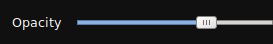
\includegraphics[height=1cm]{images/opacity-slider.png}
\caption{Trace opacity slider}
\label{opacityslider}
\end{figure}

\begin{figure}[H]
\centering
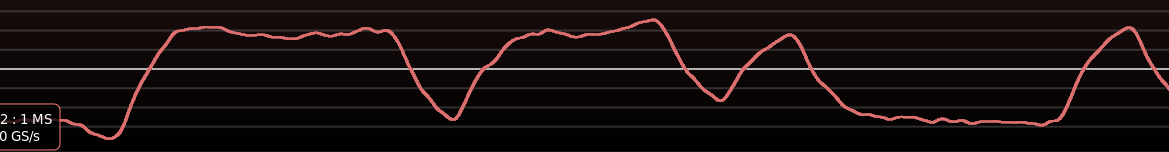
\includegraphics[width=10cm]{images/sparse-waveform.png}
\caption{Sparse waveform at a high zoom level}
\label{sparse-waveform}
\end{figure}

\begin{figure}[H]
\centering
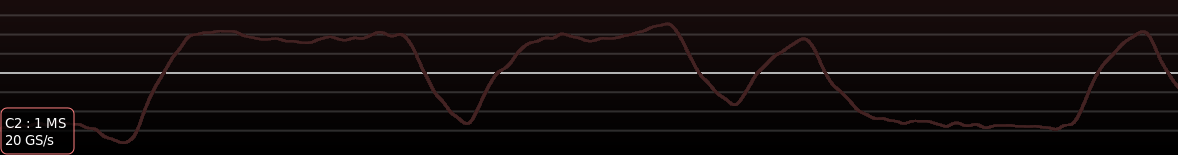
\includegraphics[width=10cm]{images/dim-waveform.png}
\caption{Dim waveform showing difficulty of seeing waveform at low opacity}
\label{dim-waveform}
\end{figure}

For example, the DVI waveform in Fig. \ref{washedout-waveform} looks like a solid white blob with a vaguely visible
outline. No fine detail can be observed other than the increased over/undershoot and random-looking edges on the
scanlines, compared to the flat appearance of the blanking period between scanlines and at the end of the frame.

When the opacity is reduced in this example, many more nuances of the signal become apparent. The high/low voltage
levels of the signal compared to the transitions between them are obvious, and the H/V sync pulses within the blanking
period show up as a slightly darker region.

\begin{figure}[H]
\centering
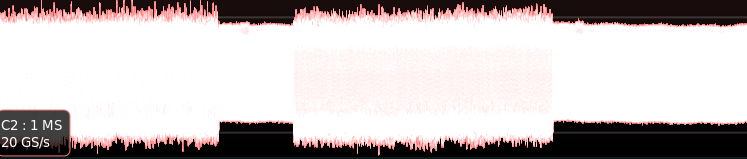
\includegraphics[width=10cm]{images/washedout-waveform.png}
\caption{Intensity-graded waveform showing washed-out appearance at high opacity}
\label{washedout-waveform}
\end{figure}

\begin{figure}[H]
\centering
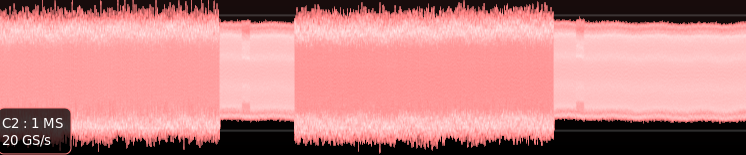
\includegraphics[width=10cm]{images/graded-waveform.png}
\caption{Intensity-graded waveform at lower opacity level}
\label{graded-waveform}
\end{figure}

As of this writing, the opacity setting is global for the entire application. Should this be changed to per waveform
group? If so, how should the group be selected and should there still be an option to make changes globally?

\FloatBarrier
\pagebreak
\section{Waveform Groups}

A waveform group is a collection of one or more waveforms stacked vertically under a common timeline. All waveforms
within a group share the same timeline and vertical cursor(s).

When glscopeclient starts up, by default all channels on the attached instruments are displayed in a single waveform
group (Figure \ref{single-group}).

\begin{figure}[h]
\centering
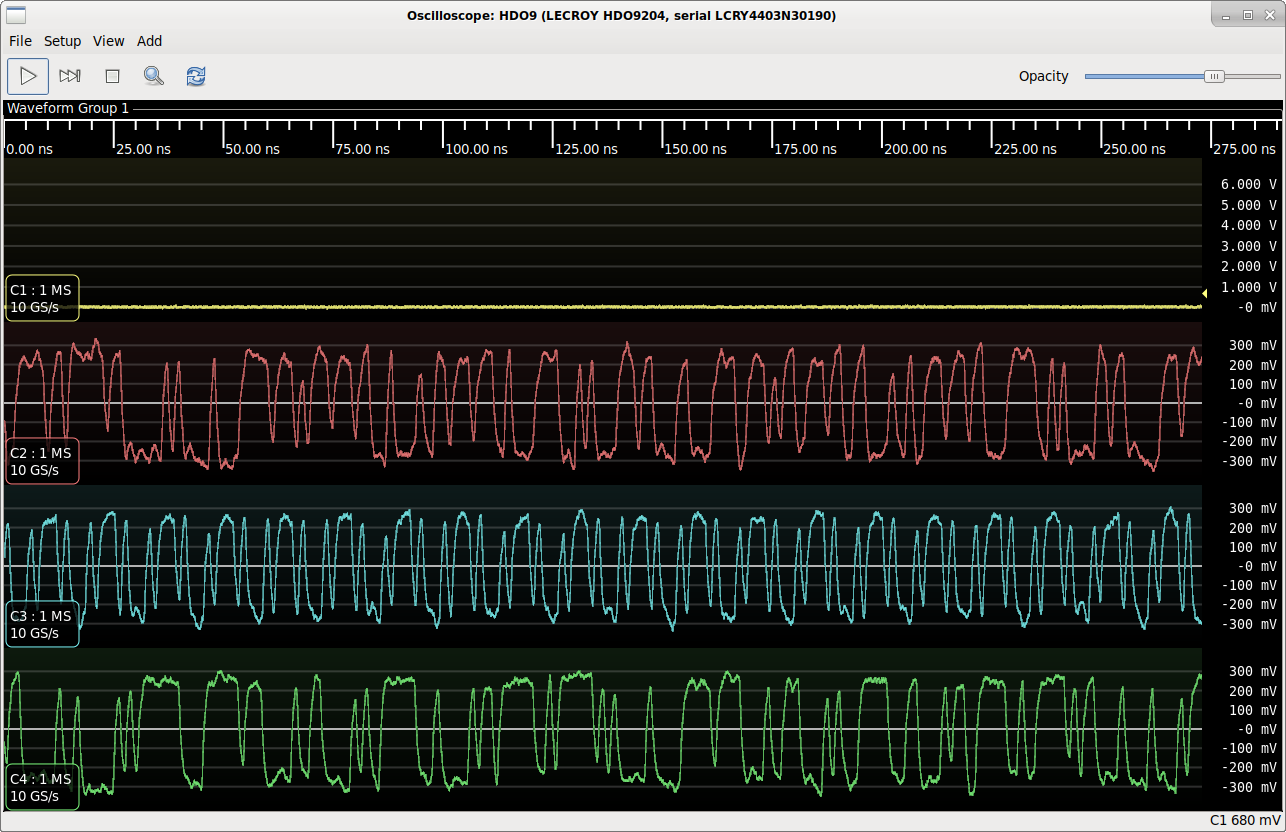
\includegraphics[width=13cm]{images/overview.png}
\caption{Top level glscopeclient window with a single waveform group}
\label{single-group}
\end{figure}

As you add protocol decodes or look at different parts of a waveform, it may be necessary to create additional waveform
groups. Typical reasons for creating additional groups include:

\begin{itemize}
\item Zooming into one set of signals to see detail on short time scales while maintaining a high level overview of
others
\item Viewing signals with incompatible horizontal units. For example, a FFT has horizontal units of frequency while an
analog waveform has horizontal units of time. Eye patterns also have horizontal units of time, but are always displayed
as two UIs wide and cannot be zoomed.
\footnote
{
It is currently possible to place signals with incompatible horizontal units in the same group. This may lead to
confusion; a future software release will likely force creation of a new group if a protocol decode is incompatible
with the parent trace's time scale.
}
\end{itemize}

\subsection{Managing Groups}

Additional groups may be created by right clicking a waveform and selecting \menustyle{[Move|Copy] waveform to / Insert
new group at [right|bottom]} from the context menu. This will split the current group's area in half horizontally or
vertically, with the selected waveform moved or copied to the newly added group and all other waveforms in the original
group.

Dividers between waveform groups may be dragged with the left mouse button. Any group may be subdivided again, to
create arbitrarily complex tiles of waveforms. Figure \ref{multiple-groups} shows a two-level hierarchy created by
moving channel 2 to a new group at right, moving channel 4 to this group, then moving channel 4 again a new group at
bottom.

\begin{figure}[h]
\centering
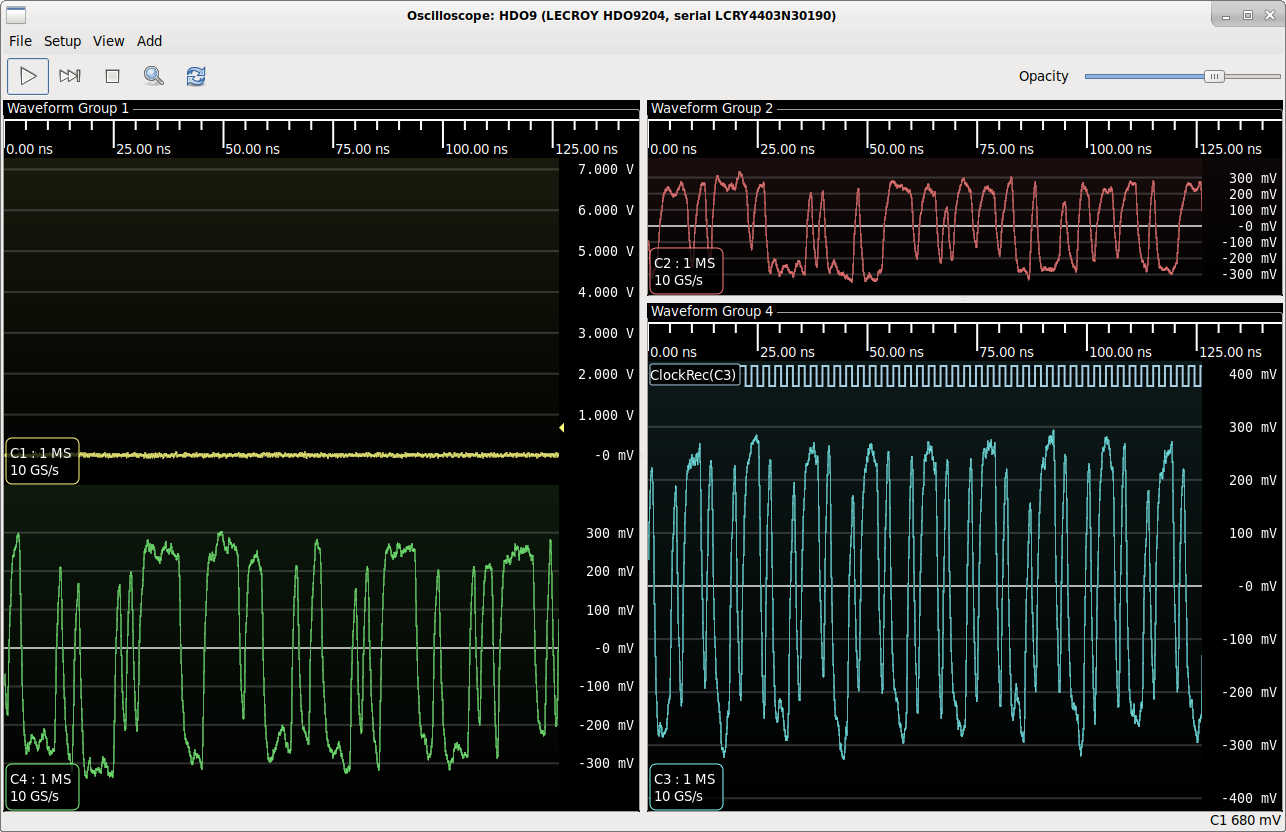
\includegraphics[width=14cm]{images/multiple-groups.png}
\caption{Top level glscopeclient window with several waveform groups separated by splitters}
\label{multiple-groups}
\end{figure}

A future software release will support using the mouse to move and copy waveforms, both between groups and within a
group (scopehal-apps:6). The exact semantics for this are not yet defined.

New waveform groups are given an automatically generated name when created, for example "Waveform Group 2". This name
will be editable in a future software release (scopehal-apps:53).

\pagebreak
\section{Timeline}

The timeline is displayed at the top of each waveform group and shows the X axis scale for the group. The timeline (and
all accompanying waveform views in the group) may be zoomed by scrolling with the mouse wheel, or panned by dragging
with the left mouse button.

Unlike classical oscilloscope user interfaces, there is \emph{no relationship} between the timeline scale/position and
the duration of the acquisition. It is possible to zoom or scroll beyond the end of the acquisition (displaying empty
background with no signal) or have a deep capture in which nearly all acquired data is offscreen.

TODO: talk about how to set trigger offset in capture and change timebase once that's implemented

TODO: insert screenshot after we have some pending UI changes done

\pagebreak
\section{Waveform Views}

A waveform view is a 2D graph of a signal or protocol decode within a waveform group.

\subsection{Plot Area}

The plot area shows the waveform being displayed. The background has a subtle gradient from light at top to dark at
bottom, in order to visually separate adjacent waveform view within the same group.

The horizontal grid lines line up with the voltage scale markings on the Y axis. If the plot area includes Y=0, the
grid line for zero is slightly brighter.

\begin{figure}[H]
\centering
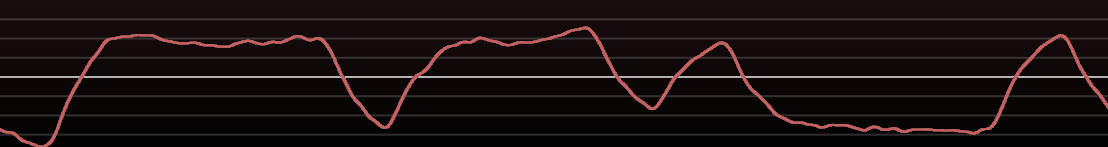
\includegraphics[width=10cm]{images/waveform-graph.png}
\caption{Waveform plot area}
\label{waveform-graph}
\end{figure}

The waveform is drawn as a semi-transparent line so that when zoomed out, the density of voltage at various points in
the graph may be seen as lighter or darker areas. This is referred to as ``intensity grading".

\begin{figure}[H]
\centering
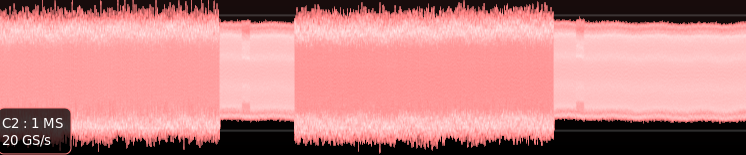
\includegraphics[width=10cm]{images/graded-waveform.png}
\caption{Intensity-graded waveform}
\label{graded-waveform2}
\end{figure}

\subsection{Y Axis Scale}

Each waveform view has its own Y axis scale, which is locked to the ADC range of the instrument.

Dragging the Y axis scale with the left mouse button currently does nothing (scopehal-apps:54) but in a future software
release will change the voltage offset of the channel.

Scrolling the Y axis scale with the mouse wheel changes the gain of the channel.

If a left-pointing arrow (as seen in Fig. \ref{y-axis}) is visible, the current channel is selected as a trigger
source. Click on the arrow and drag up or down to select the trigger level.

\begin{figure}[H]
\centering
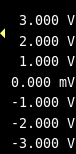
\includegraphics[height=3cm]{images/y-axis.png}
\caption{Y axis of a waveform view showing trigger arrow}
\label{y-axis}
\end{figure}

\subsection{Channel Information Box}

The channel information box is displayed in the lower left corner of each waveform view. It contains summary
information about the channel. Currently this is the display name of the channel, the sample rate, and the record
length of the acquisition. Other information, such as probe coupling, may be displayed there in the future.

Double-clicking the information box opens the channel properties dialog.

\begin{figure}[H]
\centering
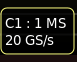
\includegraphics[width=2cm]{images/channel-infobox.png}
\caption{Channel information box}
\label{channel-infobox}
\end{figure}

\subsection{Overlays}

Waveforms may have additional information overlaid on top of them, such as protocol decodes. Each overlay has its own
information box, which may be double-clicked to open the properties dialog and configure it just like any other
channel.

Fig. \ref{overlays} shows
an example of an analog waveform with three overlays: thresholding it to NRZ digital, recovering a sampling
clock with a CDR PLL, and finally decoding the serial NRZ data stream to TMDS protocol data and control events.

\begin{figure}[H]
\centering
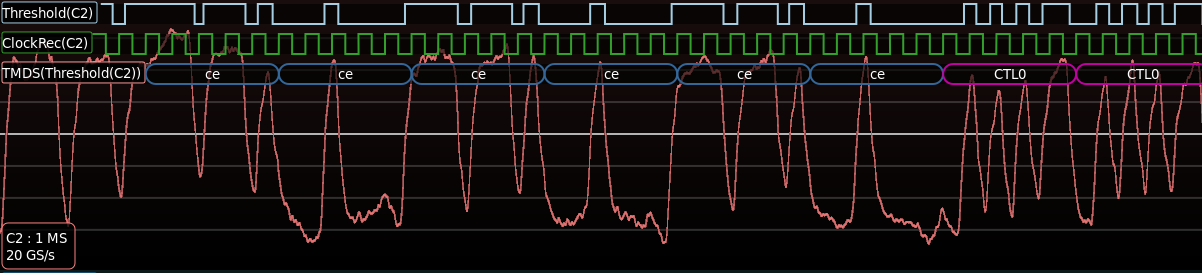
\includegraphics[width=14cm]{images/overlays.png}
\caption{Waveform showing two digital overlays and a data decode overlay}
\label{overlays}
\end{figure}

Overlays can be deleted but cannot currently be moved between waveform areas or reordered within a single waveform area
(scopehal-apps:7, scopehal-apps:6)

\pagebreak
\section{History View}
\label{sec:history}

glscopeclient has the ability to save every waveform during a session in memory, allowing you to go back in time and
see previous state of the system being debugged.

By default, the history view (Fig. \ref{historyview}) is not displayed and no history is captured. If the history view
is closed, past history is removed. (TODO: we should probably display a warning prompt or keep existing history when
doing this?)

\begin{figure}[H]
\centering
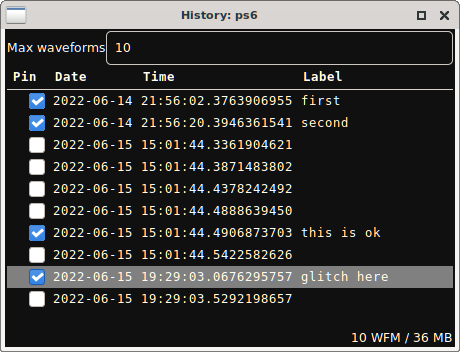
\includegraphics[width=5cm]{images/history-view.png}
\caption{Waveform history view}
\label{historyview}
\end{figure}

The ``max waveforms" box allows the depth of the history to be configured. It defaults to 100 but can be set to any
positive integer value. Older waveforms beyond the history limit are deleted as new waveforms are acquired.

The status bar at the bottom of the history view displays the total number of waveforms in the history, as well as an
estimate of the amount of RAM used by the history.

\subsection{Estimating Waveform Memory Usage}

When selecting a maximum depth for the history, it is important to pick a reasonable limit to avoid running out of RAM!
glscopeclient will happily fill tens or hundreds of gigabytes of memory with deep waveforms if given a chance. Memory
usage of waveform data can be roughly estimated as 16+sizeof(sample type) bytes per point, since each sample contains a
64-bit timestamp and duration plus the sample data.

For example, an analog sample takes 20 bytes of RAM (16 of time plus a 32-bit floating point voltage measurement) per
sample. Thus, a 1M point analog waveform takes approximately 20 MB of RAM per channel, or 80 MB per capture on a
four-channel oscilloscope with all channels enabled.

On the larger side, a 10M point four channel capture would use 800 MB and a 64M point deep-memory capture would use 5
GB. The default 100-waveform history setting is thus wildly inappropriate for such deep captures! A future software
release may support spilling waveform data to a temporary directory on disk, permitting effectively unlimited history
depth given sufficient disk space.

Digital waveforms use one byte per sample for the actual measurement, so 17 MB per channel for a 1M point waveform.

Protocol decode memory usage varies depending on the specific decode, however it is typically not a large contributor
to the overall glscopeclient RAM footprint when using history mode because decodes are evaluated dynamically each time
a waveform is pulled from history rather than having output cached for every historical waveform. Thus, at most one
copy of each decoder's output is present in memory regardless of history depth.

\pagebreak
\section{Protocol Analyzer View}

\pagebreak
\section{Protocol Decodes, Math Functions, and Measurements}

\subsection{Introduction}

\subsubsection{Key Concepts}

glscopeclient and libscopehal are based on a ``filter graph" architecture internally. The filter graph is a directed
acyclic graph with a set of source nodes (waveforms captured from hardware or loaded from a file) and sink nodes
(waveform views) connected by edges representing data flow.

A protocol decode is simply an intermediate node in the graph, which takes input from one or more waveform nodes and
outputs a waveform which may be displayed in a waveform view, used as input to other protocol decodes, or both. A
waveform is a series of data points which may represent voltages, digital samples, or arbitrarily complex protocol data
structures.

As a result, there is no internal distinction between math functions and protocol decodes, and it is possible to chain
them arbitrarily. Consider the following example\footnote{Not all of these filters are currently implemented}.

\begin{itemize}
\item Two analog waveforms representing serial data and clock are acquired
\item Each analog waveform is thresholded, producing a digital waveform
\item The two digital waveforms are decoded as $I^2C$, producing a series of packets
\item The $I^2C$ packets are decoded as writes to a serial DAC, producing an analog waveform
\item A moving average filter is applied to the analog waveform
\end{itemize}

In this document we use the term ``protocol decoder" consistently to avoid ambiguity.

\subsubsection{Conventions}

Each protocol decode takes one or more inputs (vector inputs), zero or more parameters (scalar inputs), and outputs a
signal (vector output).

If the output signal is a complex-valued type (as opposed to a single scalar, e.g. voltage, at each sample) the
``Output Signal" section will include a table describing how various types of output data are displayed. Printf-style
format codes maybe used for clarity. For example, ``\%02x" means data is formatted as hexadecimal bytes with leading
zeroes.

All protocol decodes with complex output use a standardized set of colors to display various types of data fields in a
consistent manner. These colors are currently hard coded in a table but will be made editable in the future
(scopehal-apps:43)

Suggestions on changes to the default colors, or new categories for color coding, are welcome

\begin{tabularx}{16cm}{llX}
\thickhline
\textbf{Color name} & \textbf{Use case} & \textbf{Default Color} \\
\thickhline
Address & Memory addresses & \cellcolor{address}\textcolor{black}{\#ffff00} \\
\thickhline
Checksum Bad & Incorrect CRC/checksum & \cellcolor{checksumbad}\textcolor{white}{\#ff0000} \\
\thickhline
Checksum OK & Valid CRC/checksum & \cellcolor{checksumok}\textcolor{black}{\#00ff00} \\
\thickhline
Control & Miscellaneous control data & \cellcolor{control}\textcolor{white}{\#c000a0} \\
\thickhline
Data & User data & \cellcolor{data}\textcolor{white}{\#336699} \\
\thickhline
Error & Malformed/unreadable data & \cellcolor{error}\textcolor{white}{\#ff0000} \\
\thickhline
Idle & Inter-frame gaps & \cellcolor{idle}\textcolor{white}{\#404040} \\
\thickhline
Preamble & Preamble/sync words & \cellcolor{preamble}\textcolor{white}{\#808080} \\
\thickhline
\end{tabularx}

\subsection{8B/10B (IBM)}

\subsection{8B/10B (TMDS)}

Decodes the 8-to-10 Transition Minimized Differential Signalling line code used in DVI and HDMI.

\subsubsection{Inputs}

\begin{tabularx}{16cm}{llX}
\thickhline
\textbf{Signal name} & \textbf{Type} & \textbf{Description} \\
\thickhline
data & 1-bit digital & Serial TMDS data line \\
\thickhline
clk & 1-bit digital & DDR \emph{bit} clock, typically generated by use of the \hyperref[filter:cdrpll]{Clock Recovery
(PLL)} decode on the input data. Note that this is 5x the rate of the HDMI pixel clock signal. \\
\thickhline
\end{tabularx}

\subsubsection{Parameters}

This decode takes no parameters.

\subsubsection{Output Signal}

The TMDS decode outputs a time series of TMDS sample objects. These consist of a type field and a byte of data.

The output of the TMDS decode is commonly fed to the \hyperref[filter:dvi]{DVI} or \hyperref[filter:hdmi]{HDMI}
protocol decoders.

\begin{tabularx}{16cm}{lllX}
\thickhline
\textbf{Type} & \textbf{Description} & \textbf{Color} & \textbf{Format} \\
\thickhline
Control & Control codes (H/V sync) & \cellcolor{control}\textcolor{white}{Control} & CTL\%d \\
\thickhline
Data & Pixel/island data & \cellcolor{data}\textcolor{white}{Data} & \%02x \\
\thickhline
Error & Malformed data & \cellcolor{error}\textcolor{white}{Error} & ERROR \\
\thickhline
Guard band & HDMI data/video guard band & \cellcolor{preamble}\textcolor{white}{Preamble} & GB \\
\thickhline
\end{tabularx}

\subsection{AC Couple}
\subsection{Average}
\subsection{Base}
\subsection{CAN}
\subsection{Clock Jitter (TIE)}
\subsection{Clock Recovery (PLL)}
\label{filter:cdrpll}

\subsection{Clock Recovery Debug}
\subsection{Clock Recovery (UART)}
\subsection{DC Offset}
\subsection{Difference}
\subsection{DVI}
\label{filter:dvi}

\subsection{Ethernet - 10baseT}
\subsection{Ethernet - 100baseTX}
\subsection{Ethernet Autonegotiation}
\subsection{Eye Bitrate}
\subsection{Eye Height}
\subsection{Eye Pattern}
\subsection{Eye Period}
\subsection{Eye P-P Jitter}
\subsection{Eye Width}
\subsection{Fall 80-20}
\subsection{Fall 90-10}
\subsection{Frequency}
\subsection{FFT}
\subsection{HDMI}
\label{filter:hdmi}
\subsection{$I^2C$}
\subsection{JTAG}
\subsection{Max}
\subsection{MDIO}
\subsection{Min}
\subsection{Moving Average}
\subsection{Overshoot}
\subsection{Period}
\subsection{Peak-Peak}
\subsection{Rise 10-90}
\subsection{Fall 20-80}
\subsection{Sin(x)/x Interpolation}
\subsection{Threshold}
\subsection{Top}
\subsection{UART}
\subsection{Undershoot}
\subsection{USB 1.0 / 2.x Activity}
\subsection{USB 1.0 / 2.x Packet}
\subsection{USB 1.0 / 2.x PCS}
\subsection{USB 1.0 / 2.x PMA}
\subsection{Waterfall}

\end{document}
